\chapter{Arquitetura para compartilhamento de informações do ativo}
\label{cha:arquitetura}
	
	A elaboração de uma arquitetura comum para o compartilhamento de informações do ativo é essencial para que haja consistência e interoperabilidade entre os membros da CS adotando este sistema.
	
	Esta seção tem o objetivo de apresentar detalhes da arquitetura proposta baseada em \textit{Web Services} (WS) nos modelos de uma arquitetura orientada a serviços (SOA) compatível com Componentes I4.0 para o compartilhamento de informações do ativo ao longo da CS.
	
	É apresentado também nesta seção o mapeamento dos componentes desta arquitetura dentro do eixo camadas do RAMI4.0.
	
\section{ Componentes e operações do WS }

	Um WS é um serviço disponibilizado remotamente por meio de um servidor, que escuta e responde solicitações de clientes por meio de uma determinada rede e porta. Os clientes, por sua vez, consomem o serviço disponibilizado pelo servidor por meio de solicitações.
	
	Os componentes e operações da arquitetura proposta para a comunicação entre ativos ao longo da Cadeia de Suprimentos é baseada na estrutura de um WS (vide \autoref{fig:componentes-webservice}). Esta arquitetura envolve três componentes (atores) básicos: O cliente, o servidor e o repositório; e três operações: publicação, busca e interação. 
	
	Nesta seção são apresentados detalhes sobre os componentes e operações necessárias para o fornecimento de WSs no mundo conectado da I4.0
	
\subsection{ Componentes do WS }

	Os três componentes/atores em um WS são: O Cliente, o Servidor e o repositório. Estes componentes e suas interrelações são apresentadas na \autoref{fig:aas-wb}.
	
	\begin{figure}[htb]
		\centering
		\caption{Componentes e operações do WS.}
		\label{fig:aas-wb}
		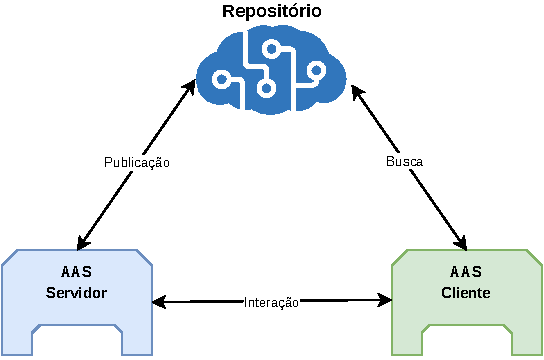
\includegraphics[width=0.7\textwidth]{aas-wb}
		\fonte{O autor.}
	\end{figure}

	De maneira sucinta, os componentes são descritos da seguinte forma: ``O AAS Servidor'' é a parte que tem um serviço a oferecer para os demais AASs no mundo conectado, o ``AAS Cliente'' é a parte que necessita de algum serviço e que age ativamente para receber este serviço e o ``Repositório'' é a parte que armazena informações sobre descrições de vários serviços.
	
	A \autoref{tab:componentes-ws} lista os componentes do WS para a I4.0 e suas respectivas descrições detalhadas.
	
	\begin{table}[htb]
		\centering
		\caption{Componentes do WS para I4.0.}
		\label{tab:componentes-ws}
		\begin{tabular}{p{3cm}p{12cm}}
			\hline
			\textbf{Componente}
			& \textbf{Descrição} \\ 
			
			\hline
			AAS Servidor
			& O AAS Servidor é a conexão direta com o ativo. Este AAS extrai e disponibiliza informações sobre o ativo para a MDP. Cada submodelo do AAS representa um conjunto de informações e serviços semelhantes agrupados. \\
			
			\hline
			AAS Cliente
			& O AAS Cliente é a parte que irá consumir as informações disponibilizadas pelo AAS Servidor. O cliente representa cada uma das partes envolvidas na cadeia de suprimentos. Pode representar uma instituição, uma pessoa física ou até mesmo uma outra máquina/produto. \\
			
			\hline
			Repositório
			& O repositório é a plataforma que recebe, armazena e disponibiliza informações de descrição sobre todos os serviços disponíveis no mundo conectado. O AAS recebe operações de ``publicação'' por parte do AAS Servidor e operações de ``busca'' por parte do AAS Cliente. O Repositório não atua como canal de comunicação entre AAS Cliente e Servidor, mas apenas fornece informações necessárias para que ambos os AAS possam se comunicar diretamente por meio da operação de ``interação''. \\
			
			\hline
		\end{tabular}
		\fonte{O autor.}
	\end{table}
	
	Neste modelo, a descrição dos serviços disponíveis nos submodelos de cada AAS é armazenada em um repositório comum, onde todos os AASs disponíveis no mundo conectado poderiam se tornar visíveis. A função do repositório é armazenar uma descrição dos serviços disponíveis e não o serviço em si. O serviço é fornecido pelo próprio AAS que o disponibilizou, servindo o repositório apenas como uma plataforma de descobertas de serviços.

	Cada AAS pode atuar tanto como um fornecedor de serviços (servidor), quanto como um solicitante de serviços (cliente), sempre usando o repositório como plataforma para descoberta.
	
	
\subsection{ Operações do WS }

	Os três tipo básicos de operações em um WS são: a publicação, a busca e a interação. A interrelação das operações com os componentes são apresentadas na \autoref{fig:aas-wb}.
	
	As operações do WS e suas descrições detalhadas são apresentadas na \autoref{tab:operacoes-ws}
	
	\begin{table}[htb]
		\centering
		\caption{Operações do WS para I4.0.}
		\label{tab:operacoes-ws}
		\begin{tabular}{p{3cm}p{12cm}}
			\hline
			\textbf{Operação}
			& \textbf{Descrição} \\ 
			
			\hline
			Publicação
			& Ação tomada pelo AAS Servidor sempre que este componente queira anunciar um serviço para que possa ser descoberto. Nesta operação, o AAS Servidor envia uma lista de seus serviços ofertados e a descrição de cada um desses serviços. Esta lista é recebida e armazenada pelo Repositório, que a disponibiliza para acesso público. \\
			
			\hline
			Busca
			& Ação tomada pelo AAS Cliente sempre que este precisa consultar serviços de seu interesse. Nesta operação o AAS Cliente faz uma solicitação ao Repositório com os parâmetros que definem o tipo e as restrições do serviço desejado. A operação de busca engloba também o fluxo contrário de informações, que é o envio da resposta da solicitação do Repositório para o AAS Cliente. \\
			
			\hline
			Interação
			& Ação tomada pelo AAS Cliente sempre que este deseja invocar um serviço. O AAS Cliente estabelece uma conexão direta com o AAS Servidor e consome o determinado serviço solicitado. A operação de interação normalmente é feita após o recebimento da lista de descrição de serviços por parte do Repositório, porém a interação pode ser feita diretamente caso o AAS Cliente já possua informações necessárias para o estabelecimento da conexão.  \\
			
			\hline
		\end{tabular}
		\fonte{O autor.}
	\end{table}
	
	Para cada uma das operações devem ser definidos protocolos padrão a fim de se garantir a interoperabilidade entre os componentes. A WSDL (\textit{Web Services Description Language}) é um documento que funciona como uma linguagem de descrição de \textit{Web Services}, que, além de descrever o serviço, especifica como acessá-lo e quais as operações ou métodos disponíveis. 
	
	A WSDL se aplica para as operações de comunicação com o repositório: publicação e busca. A WSDL estabelecerá também os padrões de comunicação suportados pelo AAS Servidor, como, por exemplo, o padrão REST ou o padrão SOAP.
	
	Quando o AAS atua como Servidor, este AAS publica a descrição de seus serviços no repositório por meio da WSDL. Quando como Cliente, o AAS busca no repositório um serviço desejado e recebe uma lista de opções de serviços com suas respectivas descrições também por meio da WSDL. Assim, o serviço mais adequado pode ser selecionado.
	
	Uma vez definido o serviço a ser consumido, o AAS Cliente estabelece a conexão direta com o AAS Servidor por meio de algum dos padrões suportados, utilizando os detalhes contidos na descrição do serviço para localizar, contactar e invocar o serviço.
	
	A \autoref{fig:pfs-ws} apresenta um diagrama PFS (\textit{Production Flow Schema}) com o fluxo ocorrência das operações básicas no WS para a I4.0.
	
	\begin{figure}[htb]
		\centering
		\caption{Diagrama PFS das operações do WS.}
		\label{fig:pfs-ws}
		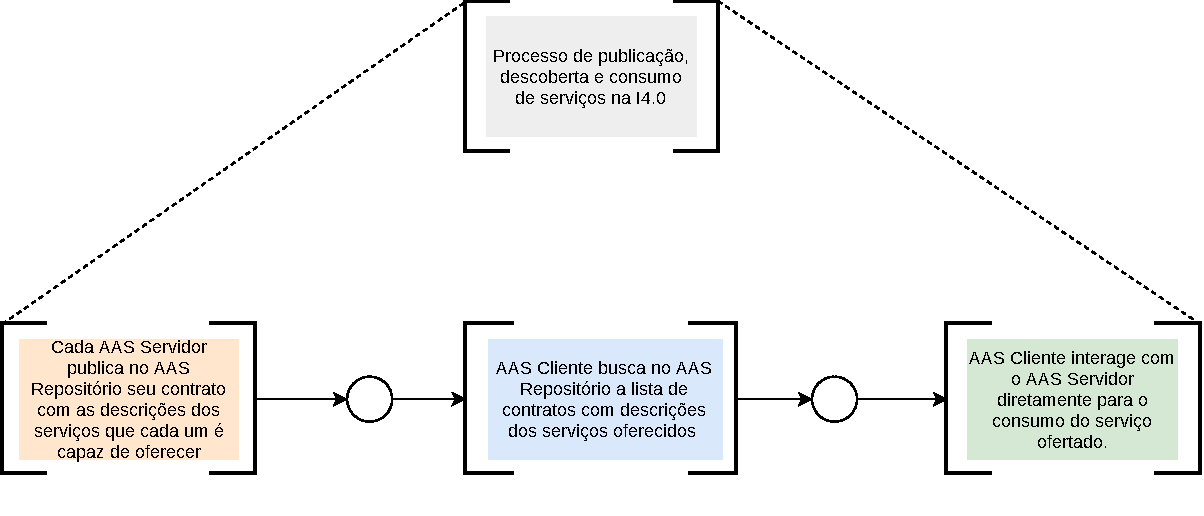
\includegraphics[width=1\textwidth]{pfs-ws}
		\fonte{O autor.}
	\end{figure}
	
	Os serviços fornecidos por um AAS são diversos, entretanto, neste trabalho serão tratados com ênfase aqueles serviços que têm como objetivo o compartilhamento de informações sobre o ativo que possam agregar valor ao produto ao longo de sua cadeia de valor. Ou seja, os serviços que extraem informações da MDP do AAS e as fornecem, mediante autenticação, às partes solicitantes ao longo da cadeia de suprimentos.

\section{Estrutura do AAS }

	Nesta proposta de arquitetura de WS, o conceito de Memória Digital do Produto (MDP) é inserido dentro da Indústria 4.0 com o objetivo de se agregar valor ao produto por meio da possibilidade de acesso a informações sobre o ativo entre parceiros ao longo da cadeia de valor.
	
	Nesta seção são apresentados os detalhes sobre a estruturação do AAS para que sejam compatíveis com a proposta de fornecimento de serviços por meio de WSs.
	
\subsection{Integração da MDP ao AAS}

	A MDP precisa ser integrada ao AAS para que possa ter a estrutura necessária para que seus dados sejam disponibilizados ao mundo conectado da I4.0. A MDP em um AAS corresponde aos dados do ativo, ao gerenciamento desses dados e às funções básicas aplicadas em cima desses dados. A MDP contém informações referentes a cada um dos submodelos em um AAS. Cada submodelo agrega informações semelhantes relativas ao ativo. 
	
	A MDP, na pratica, não estará necessariamente presente no escopo físico do ativo ao qual ela se relaciona. Como a MDP é parte integral do AAS, que representa a parte virtual do ativo, esta pode ser fornecida em qualquer meio digital, inclusive em plataformas de serviços de computação em nuvem. Estas plataformas específicas suportam o armazenamento de grandes quantidades de dados, assim como podem assegurar uma alta capacidade de processamento requisições de serviços solicitados.
	
\subsection{ Detalhamento dos componentes do AAS }

	O AAS é composto pelo cabeçalho (\textit{header}) e o corpo (\textit{body}).
	
	O cabeçalho tem a função de providenciar informações públicas sobre o ativo que o identifiquem minimamente e que forneça uma descrição sobre seus serviços oferecidos. Contém informações que podem ser acessadas sem a necessidade de autenticação, como, por exemplo, seu identificador único universal (UUID - \textit{Universal Unique IDentifier}), o modelo e fabricante do ativo. O cabeçalho contém também a descrição dos serviços fornecidos por seus submodelos. A descrição dos serviços é enviada ao repositório ou pode ser também consultada diretamente pelo AAS solicitante.
	
	A descrição de cada serviço em um cabeçalho de AAS deve necessariamente conter também referências ao AAS Servidor, ou seja, \textit{links} e identificações que permitam que o cliente possa localizar, contactar e invocar o serviço ofertado.
	
	O cabeçalho não tem a função de fornecer uma ficha técnica detalhada, mas apenas uma caracterização abstrata do ativo. Dependendo da confidencialidade do ativo, o submodelo de identificação pode apenas apresentar o UUID como informação pública. Sem o UUID, o AAS se torna inacessível para qualquer uma das partes da cadeia de suprimentos.
	
	O corpo (\textit{body}) de um AAS fornece as informações e funcionalidades sensíveis sobre o ativo, que podem ser acessadas mediante autenticação. As funcionalidades dos ativos são agrupadas em forma de submodelos, que são unidades de agrupamento de funcionalidades semelhantes, como propriedades, serviços e demais regras de negócio do ativo. Já os dados relativos aos submodelos são armazenadas e gerenciadas pela MDP, que também está localizada no corpo do AAS.
	
	O corpo do AAS representa a carga útil (\textit{payload}) do AAS, pois é a porção de informação que é de fato relevante para o cliente que consumirá os serviços ofertados.
	
	A estrutura de um AAS compatível com a arquitetura de WS proposta é apresentada na \autoref{fig:estrutura-aas}.
	
	\begin{figure}[htb]
		\centering
		\caption{Estrutura do AAS com seus submodelos e a MDP.}
		\label{fig:estrutura-aas}
		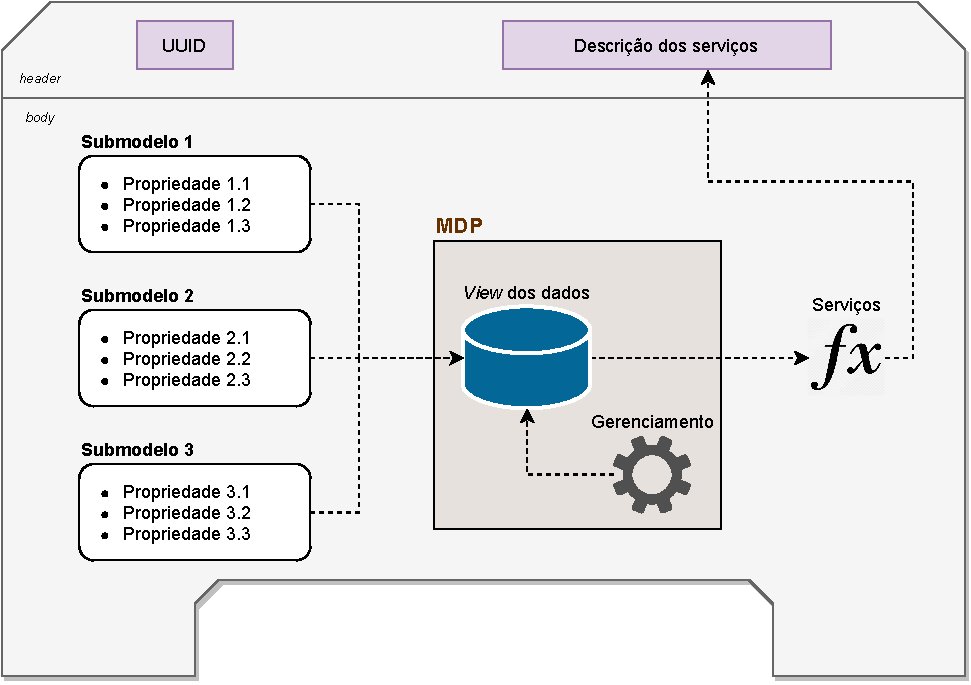
\includegraphics[width=0.7\textwidth]{estrutura-aas}
		\fonte{O autor.}
	\end{figure}

	Os dados contidos na MDP sobre submodelos, quando processados, fornecem informações sobre o ativo e agregam valor ao mesmo. Além disso, novos modelos de negócio surgem sob os dados gerados pelo ativo.
	
	Neste trabalho, é dado enfoque aos submodelos que oferecem serviços de consulta de dados a qualquer uma das partes ao longo da cadeia de suprimentos. Alguns exemplos desse tipo de submodelo podem incluir: a ficha técnica detalhada do ativo, submodelos de histórico de leitura de sensores, histórico de geolocalização do ativo, histórico de padrão de uso, etc.

\subsection{ Metamodelo dos dados da MDP}	
	
	As informações contidas na MDP devem ser estruturadas de forma tal que facilite a interpretação destes dados do lado do cliente. Para isso, metamodelos devem ser aplicados. Os metamodelos estabelecem os moldes sobre o qual devem ser elaborados os dados.
	
	Segundo \citeonline{radack2009exchangedata}, a norma IEC 61360 fornece uma estrutura e um modelo de informações no formato de dicionários de produtos. O conceito de tipo de produto é representado por ``classes'' e as características do produto são representadas por ``propriedades''.
	
	Tais propriedades são elementos de dados padronizados. As definições de tais propriedades podem ser encontradas em vários repositórios, como IEC CDD (dicionário de dados comuns) ou eCl@ss.
	
	A definição de uma propriedade associa um identificador exclusivo mundial a uma definição, que é um conjunto de atributos bem definidos. Atributos relevantes para o AAS são, entre outros, seu nome, o símbolo, a unidade de medida e uma definição textual legível para humanos da propriedade \cite{bader2019aas}.
	
	A publicação sugere formatos de transferência e armazenamento de dados. É especificado o UML (modelo neutro) e esquemas em XML e JSON, assim como mapeamentos para OPC UA, AutomationML e o \textit{Resource Description Framework} (RDF) \cite{plattform2019detailsaas}.
	
\subsection{Fluxo de fornecimento de serviços}

	As etapas para o fornecimento de serviços na I4.0 segue um fluxo padrão. A \autoref{fig:wb-funcionamento} demonstra uma exemplificação do fluxo de operações básicas de um WS em funcionamento. Neste exemplo, um AAS de um produto mantém contato com o AAS da empresa do fabricante, com o AAS da empresa do distribuidor e com o AAS do consumidor final, fornecendo o serviço de consulta de informações de diferentes submodelos para cada um dos solicitantes. 	
	
	\begin{figure}[htb]
		\centering
		\caption{Exemplificação das operações de publicação e busca.}
		\label{fig:wb-funcionamento}
		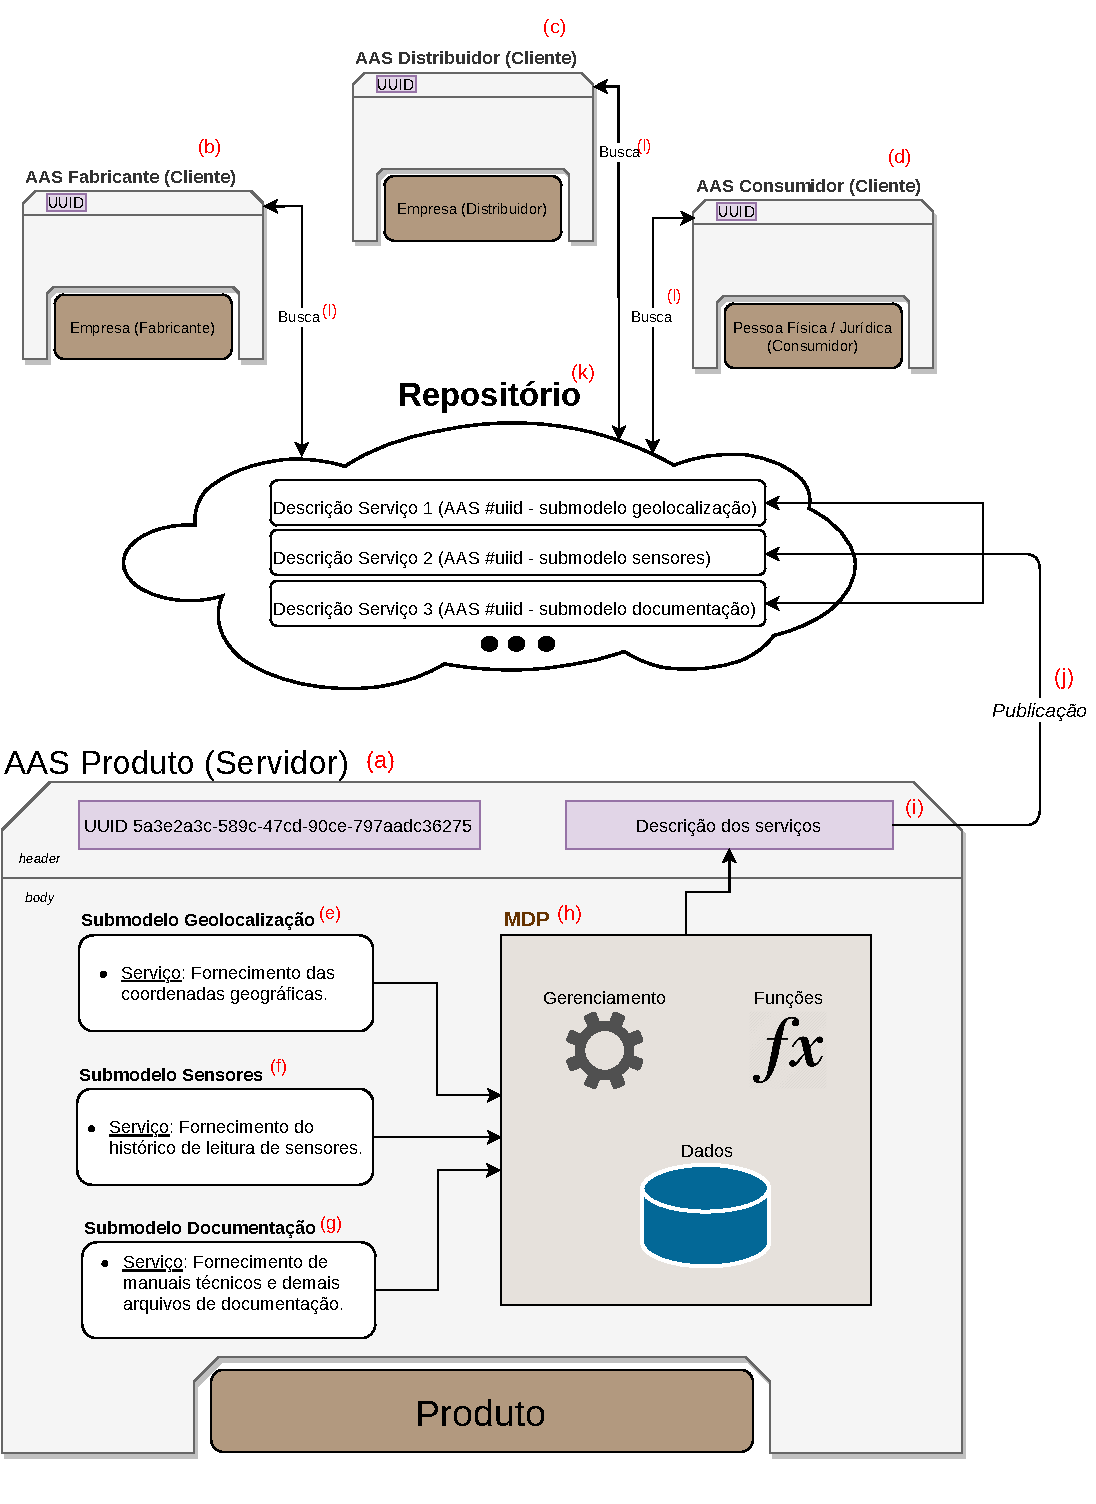
\includegraphics[width=0.8\textwidth]{wb-funcionamento}
		\fonte{O autor.}
	\end{figure}

	Neste exemplo, há três submodelos disponíveis no AAS Produto: Submodelo ``geolocalização'', submodelo ``sensores'' e submodelo ``documentação''. Os serviços de todos os submodelos disponíveis são mapeados pelas funções da MDP e, assim, é gerada uma lista de descrições de serviços. Esta lista de descrições de serviços é publicada no repositório.
	
	O repositório recebe a descrição de serviços do AAS Produto e as disponibiliza para consulta. O repositório receberá também listas de descrição de serviços de diversos outros AASs.
	
	Os AAS Clientes fazem a busca no repositório. As buscas são feitas com parâmetros a fim de se restringir qual tipo de serviço aquele cliente pretende consumir, podendo-se restringir a busca, inclusive, ao serviço de um AAS específico, identificando-o por meio de seu UUID.
	
	Cada AAS Cliente (Fabricante, Distribuidor e Consumidor), portanto, realiza a consulta ao repositório com os seus parâmetros de interesse e recebe a resposta com descrições detalhadas sobre os serviços disponíveis e informações para localizar, contactar e invocar estes serviços.
	
	O próximo passo após o recebimento da resposta do repositório é a decisão interna de cada AAS Cliente sobre qual serviço selecionar. Uma vez definido, o AAS Cliente estabelece uma comunicação direta com o AAS Servidor para o consumo do serviço selecionado.
	
	Este é um exemplo de consulta única. Em aplicações reais, o cliente normalmente invocaria o serviço de diversos AAS Servidores ao mesmo tempo, como, por exemplo, um fabricante solicitando informações de todas as máquinas de um modelo específico que foram vendidas a clientes espalhados pelo mundo para se realizar análise de dados a fim de se fazer uma manutenção preditiva e identificar possíveis falhas precocemente.
	
	Todas as atividades de invocação de serviços na fase de interação são feitas mediante autenticação. É responsabilidade das funções da MDP realizar a autenticação ou bloqueio dos serviços disponíveis de acordo com as políticas de acesso de cada AAS.
	
\section{Mapeamento das operações do WS no RAMI4.0}
	
	Segundo \citeonline{iec2017rami}, o RAMI4.0 fornece uma visão estruturada dos principais elementos de um ativo usando um modelo de níveis composto por três eixos. Desta forma, interrelações complexas podem ser divididas em seções menores e mais gerenciáveis, combinando os três eixos em cada ponto da vida do ativo para representar cada aspecto relevante.
	
	Esta seção tem o objetivo de mapear as operações do WS para dentro das camadas do RAMI4.0 de forma a representar todas as etapas do fluxo de informações em um modelo unificado.
	
	O mapeamento para o RAMI4.0, que é uma arquitetura de referência para a I4.0, contribui também para facilitar a execução de implementações do modelo de WS junto a outras soluções de I4.0, garantindo a interoperabilidades entre os sistemas.

\subsection{ Descrição das camadas do RAMI4.0 }

	A camada mais inferior, \textbf{Ativo}, é onde estão os elementos reais do Componente I4.0, como, por exemplo, máquinas, sensores, pessoas, etc; e qualquer outro elemento, físico ou não, que represente valor ao negócio.
	
	Nesta camada física estão os fornecedores de dados, ou seja, os elementos que servirão como fonte de dados. Normalmente estes dados gerados pelo ativo são extraído e monitorados a fins de controle da planta de produção. 
	
	No mundo I4.0, além de serem usados a fins de controle, podem ser usados estrategicamente para se agregar valor ao próprio ativo. Portanto, estes dados são extraídos do ativo e repassados às camadas superiores até que cheguem à Camada de Informação, onde são armazenados na MDP.
	
	Cada elemento físico deve possuir meios de comunicação e identificadores únicos (UUID), permitindo o seu monitoramento e supervisão dos dispositivos de controle por meio do AAS \cite{adolphs2015rami}.
	
	Na arquitetura proposta baseada em WSs, é possível elencar alguns componentes inclusos nessa camada, como os dispositivos físicos e os meios de sensoriamento desses dados. Outros elementos usuais dessa camada como os dispositivos de atuação e de controle também estariam inclusos, porém não se aplicam para a arquitetura de WSs.
	
	Na camada de \textbf{Integração}, estão as funcionalidade responsáveis pela virtualização de todos os ativos da camada inferior \cite{adolphs2015rami}, ou seja, a transformação de um evento real em sinais digitais. Representa a ponte entre o mundo real e o virtual.
	
	Na arquitetura proposta baseada em WSs, esta camada é relevante para o AAS Servidor, pois é dele que serão extraídos os dados desde o ativo até as camadas superiores.
	
	Esta camada contém também  as tecnologias de tranferência de dados, como o Wi-Fi, Ethernet, 5G, Bluetooth, etc.
	
	A camada \textbf{Comunicação} estabelece os protocolos de comunicação entre o dispositivo real e seu AAS, como os protocolos OPC-UA, Profinet, Profibus, etc.
	
	A camada Comunicação realiza também o pré-processamento dos dados, o que inclui a remoção de redundâncias, duplicidades e remoção de \textit{outliers}.
	
	A camada de \textbf{Informação} é onde os dados são de fato armazenados, para isso, modelos de estrutura de banco de dados são definidos de acordo os tipos de dados e suas aplicações. Alguns exemplos de estrutura de dados incluem: banco de dados relacionais (MySQL, Postgres, SQLite), banco de dados orientados a documentos (MongoDB, CouchDB), banco de dados do tipo chave-valor (Redis, Oracle NoSQL DB), etc.
	
	Esta camada é responsável por gerar e armazenar a descrição dos serviços oferecidos pelo AAS. Além disso a camada Informação contém a parte da MDP providencia os dados sob autenticação, ou seja, realiza o controle de acesso a suas informações sensíveis.
	
	Na camada \textbf{Funcional} é onde ocorre toda a interação com outros AASs contidos no mundo conectado da I4.0. Esta camada é responsável pela integração horizontal entre as partes da cadeia de suprimentos de um produto. Os serviços são disponibilizados através da camada funcional, portanto é a interface entre os AASs. 
	
	A camada Funcional define o tipo de protocolo a ser utilizado para o fornecimento dos \textit{Web Services}, o protocolo HTTP é o mais comumente adotado para o fornecimento de WSs \cite{gruner2016restful}. Alguns outros protocolos também são adotados como o MQTT, que está presente principalmente na área de automação residencial e IoT \cite{yokotani2016mqtt}.
	
	A última camada, \textbf{Regra de Negócio}, é onde estão contidas as questões legais do AAS, como as políticas de privacidade dos dados, as condições regulatórias e demais restrições aplicadas sobre os serviços.
	
	Para os WSs, outra função importante da camada Regra de Negócio é a orquestração dos serviços, que se refere ao gerenciamento dos serviços oferecidos. Quando os serviços são oferecidos em forma de contêiners, o orquestrador de serviços permite a escalabilidade da capacidade de trabalho, permitindo a invocação ou remoção de contêiners de acordo com a demanda de um determinado serviço. Alguns orquestradores de contêiners podem ser citados, como o Kubernetes, Docker Swarm e OpenShift.
	
	O conjunto de todas estas camadas representa um Componente I4.0. Para cada tipo de operação relacionada a um Componente I4.0, é necessário detalhar o fluxo de dados e de eventos acontecendo em cada uma das camadas. Este detalhamento permite que implementações de soluções I4.0 sejam facilitadas e garante que a criação dessas soluções por diversos desenvolvedores de sistemas resulte em sistemas que sejam interoperáveis, independentemente da tecnologia adotada.
	
	O Componente I4.0 pode ainda ser mais detalhadamente especificado, identificando se o componente representa um produto em desenvolvimento ou uma instância de um produto já fabricado. Estas considerações são cobertas pelo eixo Ciclo de Vida e Cadeia de Valor e considerações sobre este eixo envolvendo a arquitetura proposta baseada em WSs será apresentada no \autoref{cha:ciclo-de-vida}.
	
	A \autoref{fig:wb-rami} apresenta os componentes da arquitetura de fornecimento de WSs sob a visão das camadas do RAMI4.0. 
	
	\begin{figure}[H]
		\centering
		\caption{Camadas do RAMI4.0 com os componentes da arquitetura baseada em WSs.}
		\label{fig:wb-rami}
		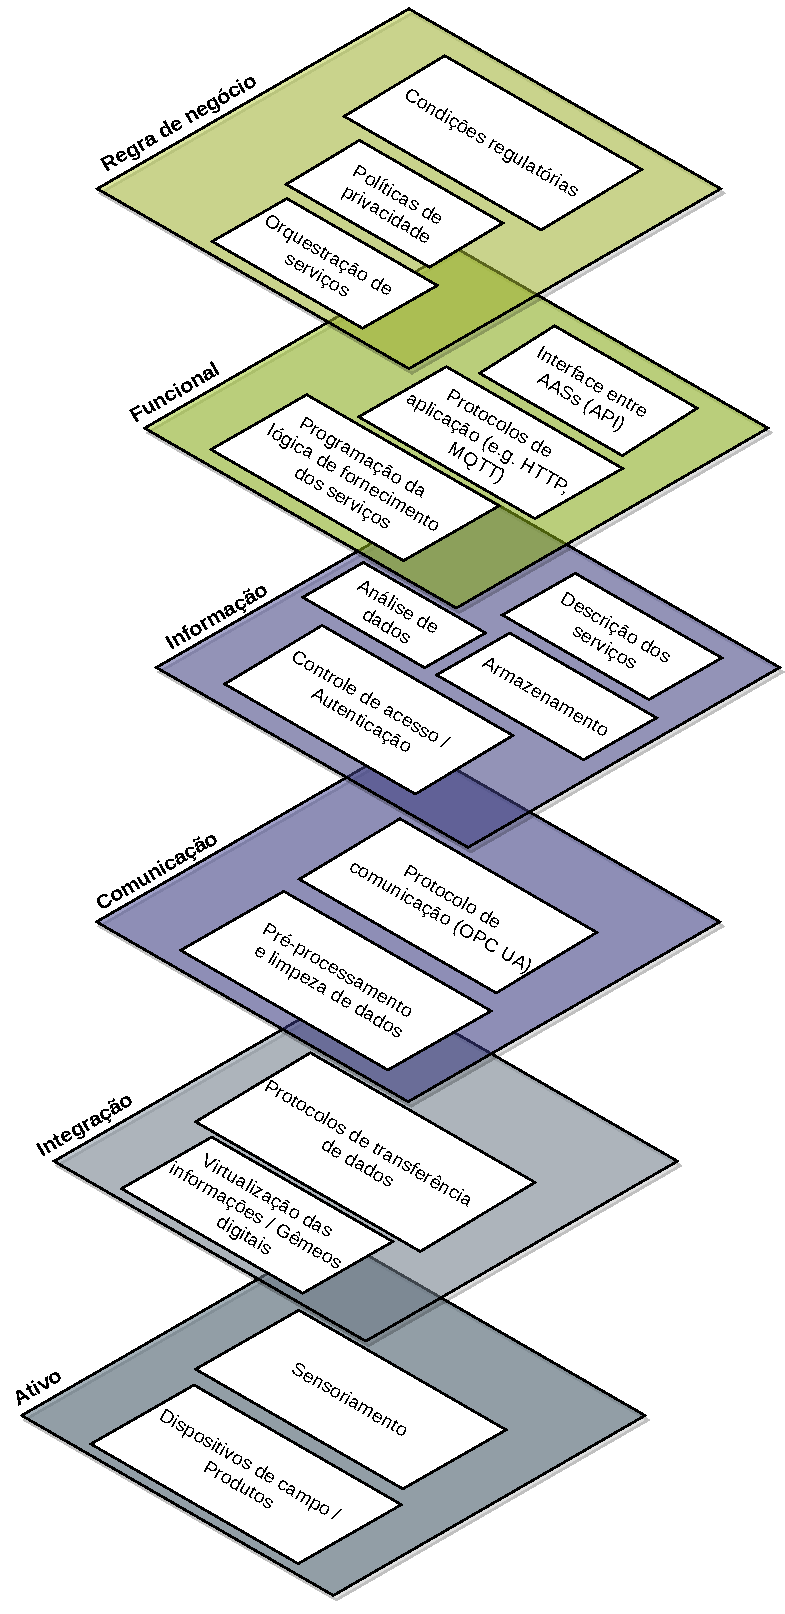
\includegraphics[height=0.9\textheight]{wb-rami}
		\fonte{O autor.}
	\end{figure}

\subsection{ Operação de Publicação }

	A \autoref{fig:rami-publicacao} apresenta diagramas PFS do fluxo de dados para a operação de publicacao de um AAS Servidor em um Repositório.
	
	\begin{figure}[htb]
		\centering
		\caption{Diagrama PFS da operação de publicação.}
		\label{fig:rami-publicacao}
		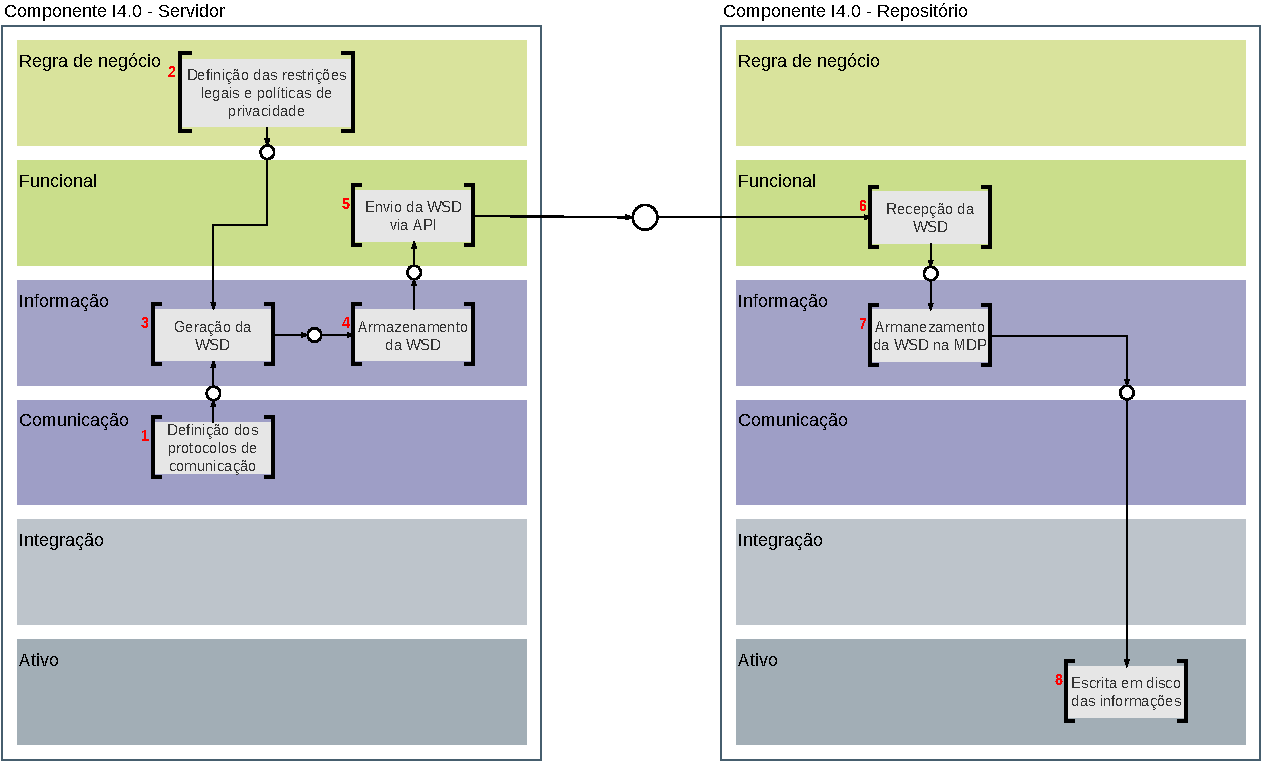
\includegraphics[width=1\textwidth]{rami-publicacao}
		\fonte{O autor.}
	\end{figure}
	

\newpage
\subsection{ Operação de Busca }

	A \autoref{fig:rami-busca} apresenta diagramas PFS do fluxo de dados para a operação de busca de um AAS Cliente e um Repositório. A operação de busca é dividida em duas partes: a requisição e a resposta.
	
	\begin{figure}[htb]
		\centering
		\caption{Diagrama PFS das duas partes da operação busca: (a) Requisição e (b) Resposta.  }
		\label{fig:rami-busca}
		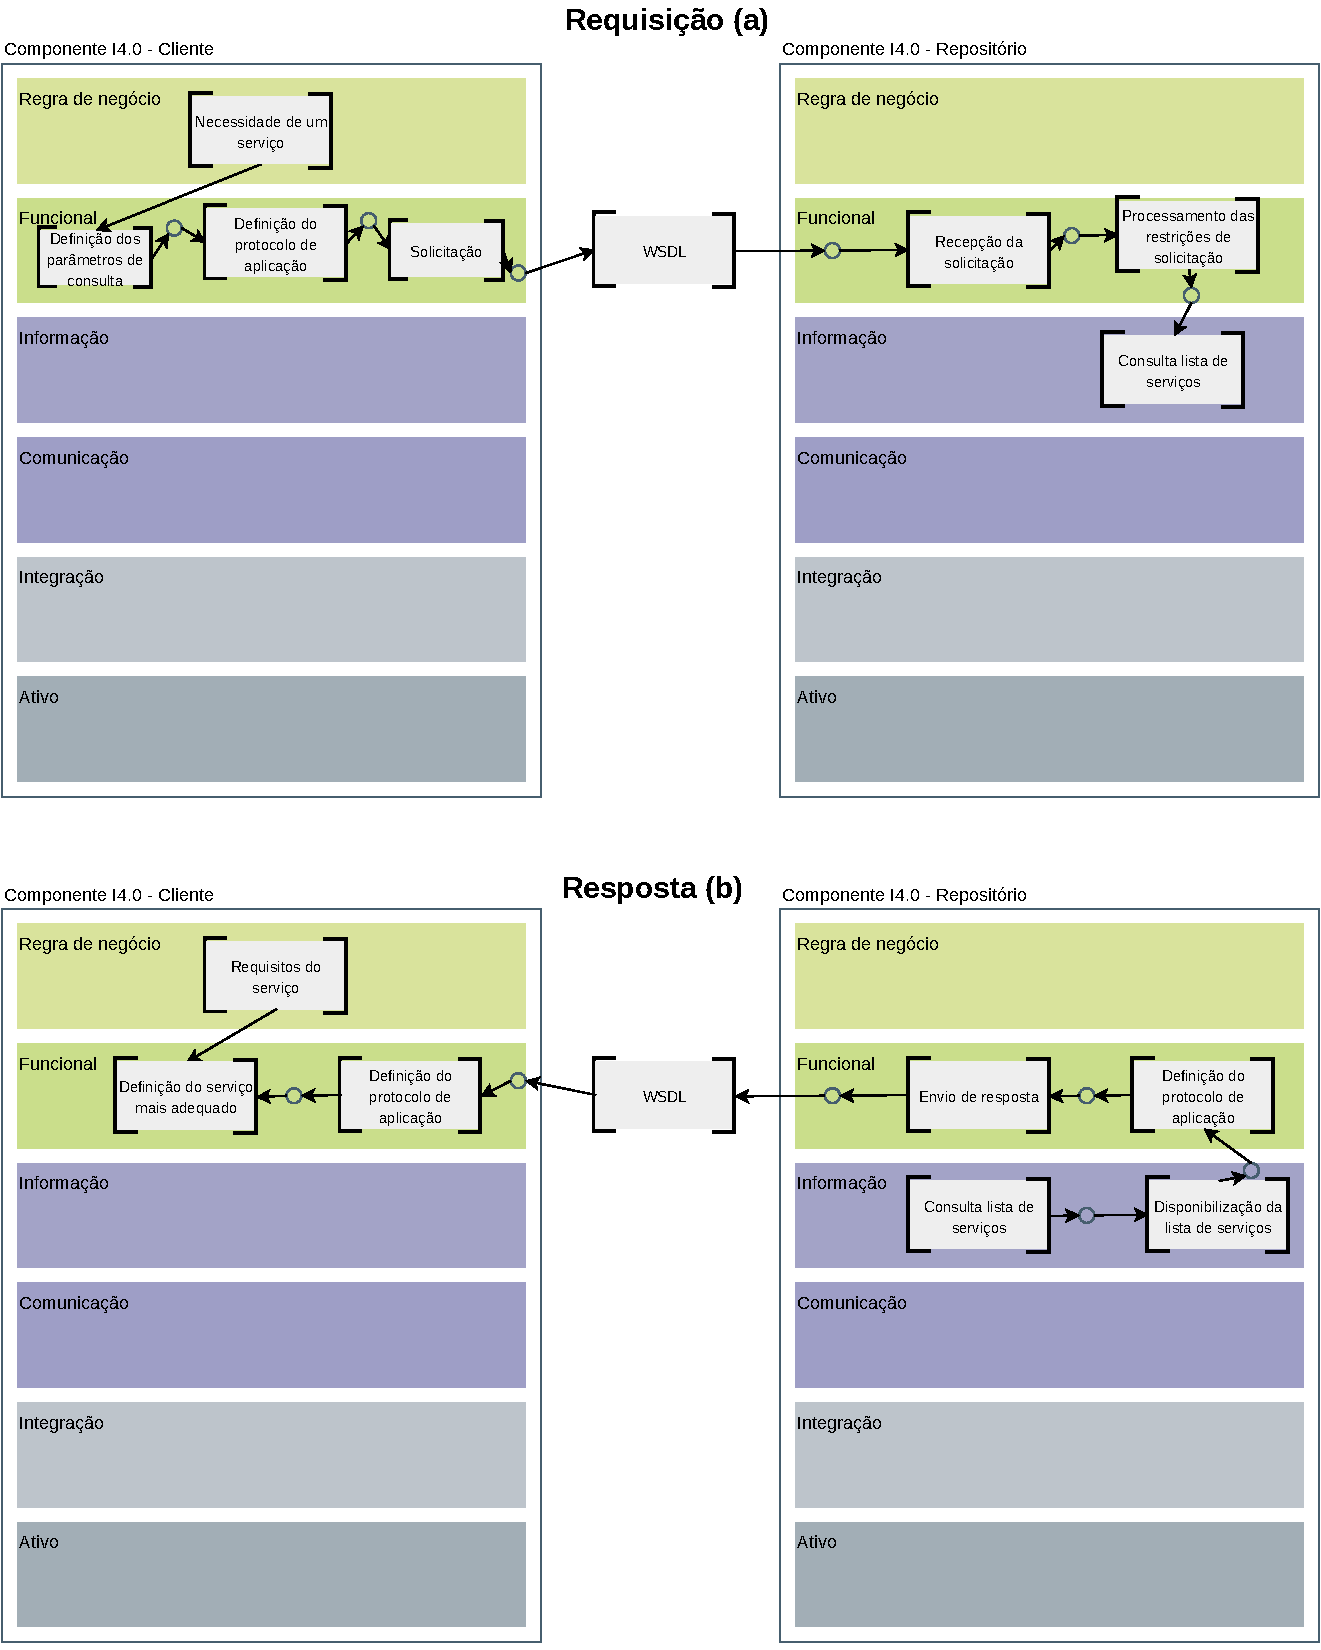
\includegraphics[width=0.9\textwidth]{rami-busca}
		\fonte{O autor.}
	\end{figure}

\newpage
\subsection{ Operação de Interação }

	A \autoref{fig:rami-interacao} apresenta diagramas PFS do fluxo de dados para a operação de interação de um AAS Servidor e um AAS Cliente.
	
	\begin{figure}[htb]
		\centering
		\caption{Diagrama PFS da operação de interação.}
		\label{fig:rami-interacao}
		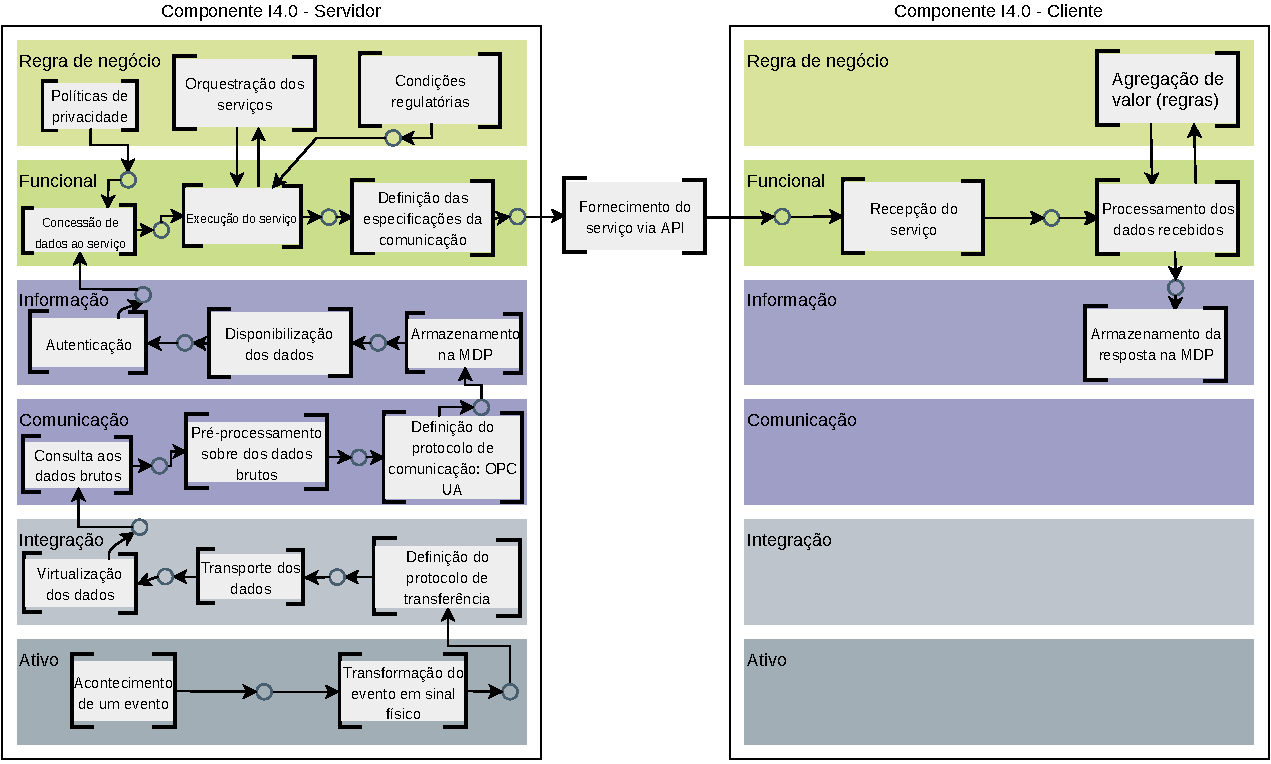
\includegraphics[width=1\textwidth]{rami-interacao}
		\fonte{O autor.}
	\end{figure}
	
